% chktex-file 2% chktex-file 29
% chktex-file 13
\documentclass[12pt]{report}
\usepackage{setspace}
\usepackage[a4paper, total={7in, 10in}]{geometry}
\usepackage[fleqn]{amsmath}
\usepackage{empheq}
\usepackage{amssymb}
\usepackage{amsthm}
\usepackage{gensymb}
\usepackage[fleqn]{cases}
\usepackage{multicol}
\usepackage{color}
\usepackage{stix}
\usepackage{chngcntr}
\usepackage{tikz}
\usepackage{enumitem}
\usepackage{pgfplots}
\usepackage{etoolbox}
\usepackage{tkz-euclide}
\usepackage{graphicx}
\usepackage{enumitem}
\usepackage{multirow}
\usepackage{mathtools}
\usepackage{mdframed}
\usepackage{adjustbox}

\def\nswe#1#2#3{#1\,$#2^\circ\,#3'$}
\graphicspath{ {./assets/} }
\usetikzlibrary{calc,trees,positioning,arrows,fit,shapes,calc, decorations.markings}
\newcommand{\midarrow}{\tikz \draw[-triangle 90] (0,0) -- +(.1,0);}

\newcommand\typel[2]{
  \mathbin{\mathop{#1\kern0pt}%
    \limits_{\raisebox{3.6ex}{\hbox to0pt{\hss\strut$\uparrow$\hss}}\hbox to0pt{\hss#2\hss}}}
}

\newcommand\typem[2]{
  \mathbin{\mathop{#1\kern0pt}%
    \limits^{\raisebox{3.6ex}{\hbox to0pt{\hss#2\hss}}\hbox to0pt{\hss\strut$\downarrow$\hss}}}
}

\counterwithout{equation}{chapter}

\newcommand{\pgfplotsdrawaxis}{\pgfplots@draw@axis}
\newcommand\perm[2][^n]{\prescript{#1\mkern-2.5mu}{}P_{#2}}
\newcommand\permtwo[2][^n]{{}_{#1}P_{#2}}
\newcommand\comb[2][^n]{{}_{#1}C_{#2}}
\newcommand\combtwo[2][^n]{\prescript{#1\mkern-2.5mu}{}C_{#2}}
\makeatother
\pgfplotsset{only axis on top/.style={axis on top=false, after end axis/.code={
          \pgfplotsset{axis line style=opaque, ticklabel style=opaque, tick style={thick,opaque},
            grid=none}\pgfplotsdrawaxis}}}

\newtheorem{theorem}{Theorem}

\mdfdefinestyle{MyFrame}{%
  linecolor=black,
  linewidth=1pt,
  roundcorner=20pt,
  innertopmargin=12pt, innerbottommargin=12pt, innerrightmargin=12pt,
  innerleftmargin=12pt, skipbelow=12pt,
  %backgroundcolor=gray!50!white}
}

\newcommand{\newitem}[1]{%
  \refstepcounter{subenum}%
  \parbox{\dimexpr.5\linewidth-.5\columnsep}{
    \makebox[\labelwidth][r]{(\thesubenum)\hspace*{\labelsep}} #1}\hfill }%%%

\setcounter{chapter}{21}

\begin{document}
\newcommand{\sol}[1]{

  \noindent \textbf{Sol.}
}
\newcommand{\prooff}[1]{

  \noindent \textbf{Proof.}
}

\newcommand{\sxrightarrow}[2][]{%
  \mathrel{\text{$\xrightarrow[#1]{#2}$}}%
}

\newenvironment{cequation}{
  \makeatletter
  \setbool{@fleqn}{false}
  \makeatother
  \begin{equation*}
    }{\end{equation*}}

\begin{titlepage}
  \raggedleft{}
  \rule{1pt}{\textheight}
  \hspace{0.02\textwidth}
  \parbox[b]{0.75\textwidth}{

  {\fontsize{40}{60}\selectfont\bfseries Mathematics}\\[2\baselineskip]
  {\huge\textit{Senior 3 Part I}}\\[4\baselineskip]
  {\Large\textsc{Melvin Chia}}

  \vspace{0.5\textheight}

  {\noindent Started on 10 April 2023}\\[\baselineskip]
  {\noindent Finished on XX XX 2023}\\[\baselineskip]
  {\noindent Actual time spent: XX days}\\[\baselineskip]}

\end{titlepage}

\chapter*{Introduction}
\addcontentsline{toc}{chapter}{Introduction} \markboth{INTRODUCTION}{}

\doublespacing{}
\section*{Why this book?}

\section*{Disclaimer}
\section*{Acknowledgements}

\singlespacing{}

\doublespacing{}
\tableofcontents
\singlespacing{}
\newpage

\setstretch{1.5}

\chapter{Function}

\section{Definition of a Function}
\subsection*{Mapping, Preimage and Image}

\begin{multicols}{2}

  For two non-empty sets $A$ and $B$, If an element $a$ inside set $A$ has a
  corresponding element $b$ inside set $B$, denoted as $a \to b$, then we say
  that $a$ is mapped to $b$ or $a$ and $b$ are paired. The mapping between two
  sets is normally denoted as $f$, $g$, $h$, etc. The mapping shown in the
  diagram below can be denoted as $f:1 \to x,\ 2 \to y,\ 4 \to z$.
  \begin{center}
    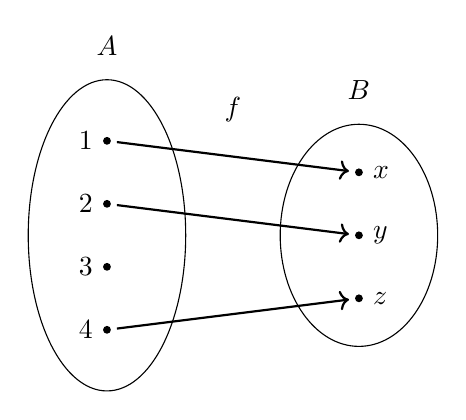
\begin{tikzpicture}[scale=0.8, ele/.style={fill=black,circle,minimum width=.8pt,inner sep=1pt},every fit/.style={ellipse,draw,inner sep=4pt}]
      \node[ele,label=left:$1$] (a1) at (0,4) {};
      \node[ele,label=left:$2$] (a2) at (0,3) {};
      \node[ele,label=left:$3$] (a3) at (0,2) {};
      \node[ele,label=left:$4$] (a4) at (0,1) {};

      \node[ele,,label=right:$z$] (b3) at (4,1.5) {};
      \node[ele,,label=right:$y$] (b2) at (4,2.5) {};
      \node[ele,,label=right:$x$] (b1) at (4,3.5) {};

      \node[draw,fit= (a1) (a2) (a3) (a4),minimum width=2cm] {} ;
      \node[draw,fit= (b1) (b2) (b3),minimum width=2cm] {} ;
      \draw[->,thick,shorten <=2pt,shorten >=2] (a1) -- (b1);
      \draw[->,thick,shorten <=2pt,shorten >=2] (a2) -- (b2);
      \draw[->,thick,shorten <=2pt,shorten >=2] (a4) -- (b3);
      \node at (2,4.5) {$f$};
      \node at (0,5.5) {$A$};
      \node at (4,4.8) {$B$};
    \end{tikzpicture}
  \end{center}
\end{multicols}

Let $f:A \to B$ is a mapping, $a$ is an element in $A$. If $a$ is mapped to $b$
under the mapping $f$, then $b$ is said to be the image of $a$ under the
mapping $f$, denoted as $b = f(a)$; $a$ is said to be the preimage of $b$ under
the mapping $f$. In the diagram above, under the mapping $f$, the image of $1$,
$2$, and $4$ are $x$, $y$, and $z$ respectively, while the preimage of $x$,
$y$, and $z$ are $1$, $2$, and $4$ respectively.

\begin{mdframed}[style=MyFrame]
  Let $A$ and $B$ be two non-empty sets, $f$ is a mapping from $A$ to $B$ such that for all elements in $A$, there is a unique corresponding element in $B$, then $f$ is a function or a mapping from $A$ to $B$, denoted as $f:A \to B$.
\end{mdframed}

The mapping shown in the diagram below is a function.
\begin{center}
  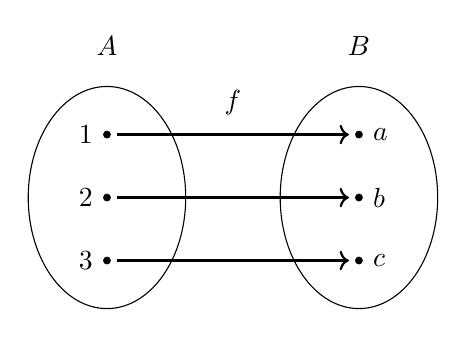
\begin{tikzpicture}[scale=0.8, ele/.style={fill=black,circle,minimum width=.8pt,inner sep=1pt},every fit/.style={ellipse,draw,inner sep=4pt}]
    \node[ele,label=left:$1$] (a1) at (0,4) {};
    \node[ele,label=left:$2$] (a2) at (0,3) {};
    \node[ele,label=left:$3$] (a3) at (0,2) {};

    \node[ele,,label=right:$c$] (b3) at (4,2) {};
    \node[ele,,label=right:$b$] (b2) at (4,3) {};
    \node[ele,,label=right:$a$] (b1) at (4,4) {};

    \node[draw,fit= (a1) (a2) (a3),minimum width=2cm] {} ;
    \node[draw,fit= (b1) (b2) (b3),minimum width=2cm] {} ;
    \draw[->,thick,shorten <=2pt,shorten >=2] (a1) -- (b1);
    \draw[->,thick,shorten <=2pt,shorten >=2] (a2) -- (b2);
    \draw[->,thick,shorten <=2pt,shorten >=2] (a3) -- (b3);
    \node at (2,4.5) {$f$};
    \node at (0,5.4) {$A$};
    \node at (4,5.4) {$B$};
  \end{tikzpicture}
\end{center}

\subsection*{Practice 1}

\setlength{\columnseprule}{1pt}
\setlength{\columnsep}{24pt}

\begin{multicols}{2}

  \begin{enumerate}
    \item For the following mappings, list the image of each element in $A$ and the
          preimage of each element in $B$, and determine whether the mapping is a
          function or not:
          \begin{enumerate}[]
            \item \adjustbox{valign=t}{
                    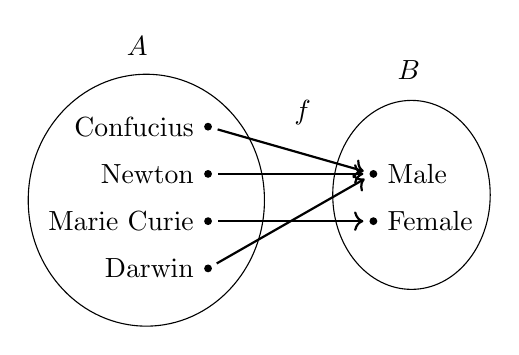
\begin{tikzpicture}[scale=0.6, ele/.style={fill=black,circle,minimum width=.8pt,inner sep=1pt},every fit/.style={ellipse,draw,inner sep=4pt}]
                      \node[ele,label=left:Confucius] (a1) at (0.5,4) {};
                      \node[ele,label=left:Newton] (a2) at (0.5,3) {};
                      \node[ele,label=left:Marie Curie] (a3) at (0.5,2) {};
                      \node[ele,label=left:Darwin] (a4) at (0.5,1) {};
                      \node[label=left:] (a999) at (-2,1) {};

                      \node[ele,,label=right:Female] (b2) at (4,2) {};
                      \node[ele,,label=right:Male] (b1) at (4,3) {};
                      \node[] (b999) at (5.5,3) {};

                      \node[draw,fit= (a1) (a2) (a3) (a4) (a999),minimum width=3cm] {} ;
                      \node[draw,fit= (b1) (b2) (b999),minimum width=2cm, minimum height=2.4cm] {} ;
                      \draw[->,thick,shorten <=2pt,shorten >=2] (a1) -- (b1);
                      \draw[->,thick,shorten <=2pt,shorten >=2] (a2) -- (b1);
                      \draw[->,thick,shorten <=2pt,shorten >=2] (a3) -- (b2);
                      \draw[->,thick,shorten <=2pt,shorten >=2] (a4) -- (b1);
                      \node at (2.5,4.3) {$f$};
                      \node at (-1,5.7) {$A$};
                      \node at (4.75,5.2) {$B$};
                    \end{tikzpicture}
                  }

            \item \adjustbox{valign=t}{
                    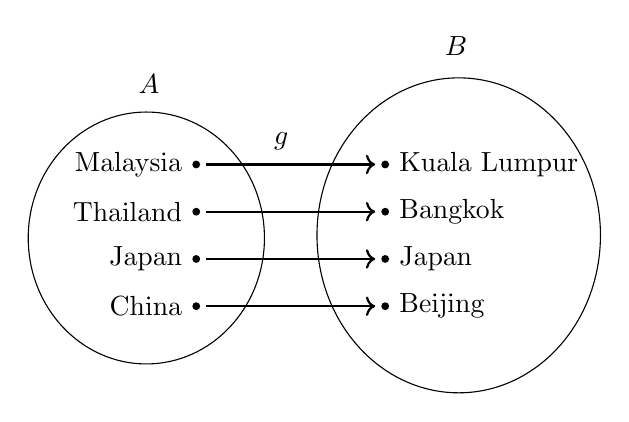
\begin{tikzpicture}[scale=0.6, ele/.style={fill=black,circle,minimum width=.8pt,inner sep=1pt},every fit/.style={ellipse,draw,inner sep=4pt}]
                      \node[ele,label=left:Malaysia] (a1) at (0,4) {};
                      \node[ele,label=left:Thailand] (a2) at (0,3) {};
                      \node[ele,label=left:Japan] (a3) at (0,2) {};
                      \node[ele,label=left:China] (a4) at (0,1) {};
                      \node[label=left:] (a999) at (-2,1) {};

                      \node[ele,,label=right:Kuala Lumpur] (b1) at (4,4) {};
                      \node[ele,,label=right:Bangkok] (b2) at (4,3) {};
                      \node[ele,,label=right:Japan] (b3) at (4,2) {};
                      \node[ele,,label=right:Beijing] (b4) at (4,1) {};
                      \node[] (b999) at (7,3) {};

                      \node[draw,fit= (a1) (a2) (a3) (a4) (a999),minimum width=3cm] {} ;
                      \node[draw,fit= (b1) (b2) (b3) (b4) (b999),minimum width=3.6cm, minimum height=4cm] {} ;
                      \draw[->,thick,shorten <=2pt,shorten >=2] (a1) -- (b1);
                      \draw[->,thick,shorten <=2pt,shorten >=2] (a2) -- (b2);
                      \draw[->,thick,shorten <=2pt,shorten >=2] (a3) -- (b3);
                      \draw[->,thick,shorten <=2pt,shorten >=2] (a4) -- (b4);
                      \node at (1.8,4.5) {$g$};
                      \node at (-1,5.7) {$A$};
                      \node at (5.5,6.5) {$B$};
                    \end{tikzpicture}
                  }

            \item \adjustbox{valign=t}{
                    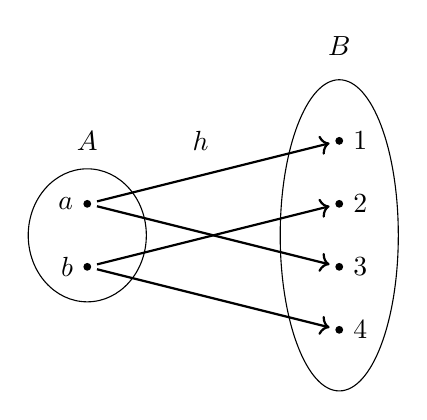
\begin{tikzpicture}[scale=0.8, ele/.style={fill=black,circle,minimum width=.8pt,inner sep=1pt},every fit/.style={ellipse,draw,inner sep=4pt}]
                      \node[ele,label=left:$a$] (a1) at (0,3) {};
                      \node[ele,label=left:$b$] (a2) at (0,2) {};

                      \node[ele,,label=right:$1$] (b1) at (4,4) {};
                      \node[ele,,label=right:$2$] (b2) at (4,3) {};
                      \node[ele,,label=right:$3$] (b3) at (4,2) {};
                      \node[ele,,label=right:$4$] (b4) at (4,1) {};

                      \node[draw,fit= (a1) (a2),minimum width=1.5cm] {} ;
                      \node[draw,fit= (b1) (b2) (b3) (b4),minimum width=1.5cm] {} ;
                      \draw[->,thick,shorten <=2pt,shorten >=2] (a1) -- (b1);
                      \draw[->,thick,shorten <=2pt,shorten >=2] (a2) -- (b2);
                      \draw[->,thick,shorten <=2pt,shorten >=2] (a1) -- (b3);
                      \draw[->,thick,shorten <=2pt,shorten >=2] (a2) -- (b4);
                      \node at (1.8,4) {$h$};
                      \node at (0,4) {$A$};
                      \node at (4,5.5) {$B$};
                    \end{tikzpicture}
                  }

            \item \adjustbox{valign=t}{
                    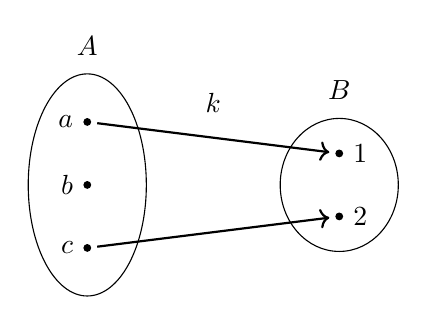
\begin{tikzpicture}[scale=0.8, ele/.style={fill=black,circle,minimum width=.8pt,inner sep=1pt},every fit/.style={ellipse,draw,inner sep=4pt}]
                      \node[ele,label=left:$a$] (a1) at (0,3) {};
                      \node[ele,label=left:$b$] (a2) at (0,2) {};
                      \node[ele,label=left:$c$] (a3) at (0,1) {};

                      \node[ele,,label=right:$1$] (b1) at (4,2.5) {};
                      \node[ele,,label=right:$2$] (b2) at (4,1.5) {};

                      \node[draw,fit= (a1) (a2) (a3),minimum width=1.5cm] {} ;
                      \node[draw,fit= (b1) (b2),minimum width=1.5cm] {} ;
                      \draw[->,thick,shorten <=2pt,shorten >=2] (a1) -- (b1);
                      \draw[->,thick,shorten <=2pt,shorten >=2] (a3) -- (b2);
                      \node at (2,3.3) {$k$};
                      \node at (0,4.2) {$A$};
                      \node at (4,3.5) {$B$};
                    \end{tikzpicture}
                  }
          \end{enumerate}

    \item Given a mapping $g:x \to x+3$, $x \in\big\{$-2, -1, 0, 1, 2, 3$\big\}$, find
          the image of each $x$.

    \item Determine whether the following mappings are functions.
          \begin{enumerate}
            \item \adjustbox{valign=t}{
                    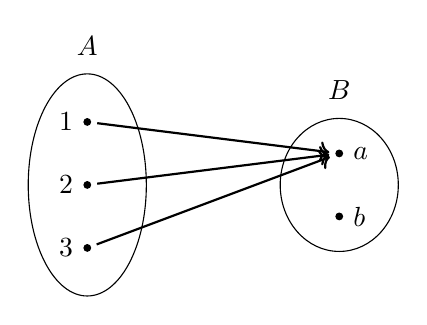
\begin{tikzpicture}[scale=0.8, ele/.style={fill=black,circle,minimum width=.8pt,inner sep=1pt},every fit/.style={ellipse,draw,inner sep=4pt}]
                      \node[ele,label=left:$1$] (a1) at (0,3) {};
                      \node[ele,label=left:$2$] (a2) at (0,2) {};
                      \node[ele,label=left:$3$] (a3) at (0,1) {};

                      \node[ele,,label=right:$a$] (b1) at (4,2.5) {};
                      \node[ele,,label=right:$b$] (b2) at (4,1.5) {};

                      \node[draw,fit= (a1) (a2) (a3),minimum width=1.5cm] {} ;
                      \node[draw,fit= (b1) (b2),minimum width=1.5cm] {} ;
                      \draw[->,thick,shorten <=2pt,shorten >=2] (a1) -- (b1);
                      \draw[->,thick,shorten <=2pt,shorten >=2] (a2) -- (b1);
                      \draw[->,thick,shorten <=2pt,shorten >=2] (a3) -- (b1);
                      \node at (0,4.2) {$A$};
                      \node at (4,3.5) {$B$};
                    \end{tikzpicture}
                  }

            \item \adjustbox{valign=t}{
                    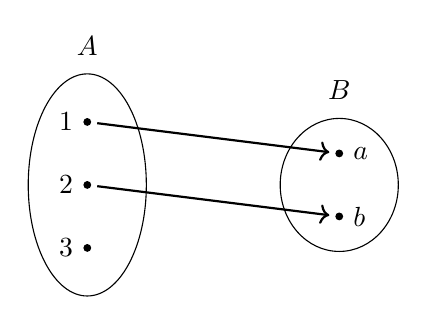
\begin{tikzpicture}[scale=0.8, ele/.style={fill=black,circle,minimum width=.8pt,inner sep=1pt},every fit/.style={ellipse,draw,inner sep=4pt}]
                      \node[ele,label=left:$1$] (a1) at (0,3) {};
                      \node[ele,label=left:$2$] (a2) at (0,2) {};
                      \node[ele,label=left:$3$] (a3) at (0,1) {};

                      \node[ele,,label=right:$a$] (b1) at (4,2.5) {};
                      \node[ele,,label=right:$b$] (b2) at (4,1.5) {};

                      \node[draw,fit= (a1) (a2) (a3),minimum width=1.5cm] {} ;
                      \node[draw,fit= (b1) (b2),minimum width=1.5cm] {} ;
                      \draw[->,thick,shorten <=2pt,shorten >=2] (a1) -- (b1);
                      \draw[->,thick,shorten <=2pt,shorten >=2] (a2) -- (b2);
                      \node at (0,4.2) {$A$};
                      \node at (4,3.5) {$B$};
                    \end{tikzpicture}
                  }

            \item \adjustbox{valign=t}{
                    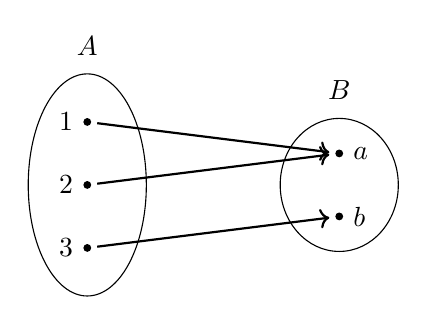
\begin{tikzpicture}[scale=0.8, ele/.style={fill=black,circle,minimum width=.8pt,inner sep=1pt},every fit/.style={ellipse,draw,inner sep=4pt}]
                      \node[ele,label=left:$1$] (a1) at (0,3) {};
                      \node[ele,label=left:$2$] (a2) at (0,2) {};
                      \node[ele,label=left:$3$] (a3) at (0,1) {};

                      \node[ele,,label=right:$a$] (b1) at (4,2.5) {};
                      \node[ele,,label=right:$b$] (b2) at (4,1.5) {};

                      \node[draw,fit= (a1) (a2) (a3),minimum width=1.5cm] {} ;
                      \node[draw,fit= (b1) (b2),minimum width=1.5cm] {} ;
                      \draw[->,thick,shorten <=2pt,shorten >=2] (a1) -- (b1);
                      \draw[->,thick,shorten <=2pt,shorten >=2] (a2) -- (b1);
                      \draw[->,thick,shorten <=2pt,shorten >=2] (a3) -- (b2);
                      \node at (0,4.2) {$A$};
                      \node at (4,3.5) {$B$};
                    \end{tikzpicture}
                  }

            \item \adjustbox{valign=t}{
                    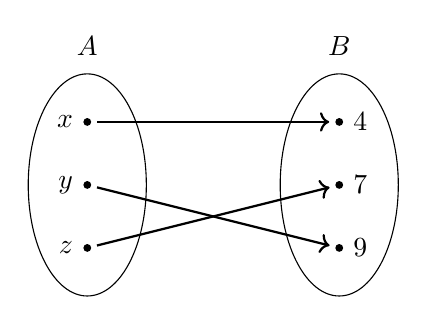
\begin{tikzpicture}[scale=0.8, ele/.style={fill=black,circle,minimum width=.8pt,inner sep=1pt},every fit/.style={ellipse,draw,inner sep=4pt}]
                      \node[ele,label=left:$x$] (a1) at (0,3) {};
                      \node[ele,label=left:$y$] (a2) at (0,2) {};
                      \node[ele,label=left:$z$] (a3) at (0,1) {};

                      \node[ele,,label=right:$4$] (b1) at (4,3) {};
                      \node[ele,,label=right:$7$] (b2) at (4,2) {};
                      \node[ele,,label=right:$9$] (b3) at (4,1) {};

                      \node[draw,fit= (a1) (a2) (a3),minimum width=1.5cm] {} ;
                      \node[draw,fit= (b1) (b2) (b3),minimum width=1.5cm] {} ;
                      \draw[->,thick,shorten <=2pt,shorten >=2] (a1) -- (b1);
                      \draw[->,thick,shorten <=2pt,shorten >=2] (a2) -- (b3);
                      \draw[->,thick,shorten <=2pt,shorten >=2] (a3) -- (b2);
                      \node at (0,4.2) {$A$};
                      \node at (4,4.2) {$B$};
                    \end{tikzpicture}
                  }

            \item \adjustbox{valign=t}{
                    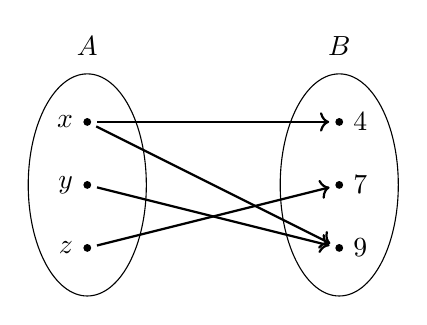
\begin{tikzpicture}[scale=0.8, ele/.style={fill=black,circle,minimum width=.8pt,inner sep=1pt},every fit/.style={ellipse,draw,inner sep=4pt}]
                      \node[ele,label=left:$x$] (a1) at (0,3) {};
                      \node[ele,label=left:$y$] (a2) at (0,2) {};
                      \node[ele,label=left:$z$] (a3) at (0,1) {};

                      \node[ele,,label=right:$4$] (b1) at (4,3) {};
                      \node[ele,,label=right:$7$] (b2) at (4,2) {};
                      \node[ele,,label=right:$9$] (b3) at (4,1) {};

                      \node[draw,fit= (a1) (a2) (a3),minimum width=1.5cm] {} ;
                      \node[draw,fit= (b1) (b2) (b3),minimum width=1.5cm] {} ;
                      \draw[->,thick,shorten <=2pt,shorten >=2] (a1) -- (b1);
                      \draw[->,thick,shorten <=2pt,shorten >=2] (a1) -- (b3);
                      \draw[->,thick,shorten <=2pt,shorten >=2] (a2) -- (b3);
                      \draw[->,thick,shorten <=2pt,shorten >=2] (a3) -- (b2);
                      \node at (0,4.2) {$A$};
                      \node at (4,4.2) {$B$};
                    \end{tikzpicture}
                  }

            \item \adjustbox{valign=t}{
                    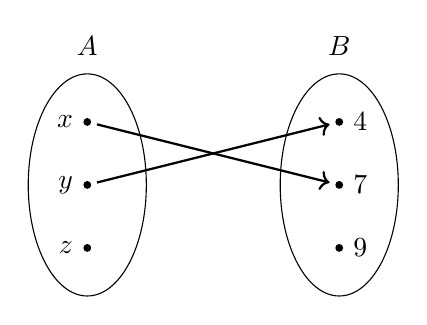
\begin{tikzpicture}[scale=0.8, ele/.style={fill=black,circle,minimum width=.8pt,inner sep=1pt},every fit/.style={ellipse,draw,inner sep=4pt}]
                      \node[ele,label=left:$x$] (a1) at (0,3) {};
                      \node[ele,label=left:$y$] (a2) at (0,2) {};
                      \node[ele,label=left:$z$] (a3) at (0,1) {};

                      \node[ele,,label=right:$4$] (b1) at (4,3) {};
                      \node[ele,,label=right:$7$] (b2) at (4,2) {};
                      \node[ele,,label=right:$9$] (b3) at (4,1) {};

                      \node[draw,fit= (a1) (a2) (a3),minimum width=1.5cm] {} ;
                      \node[draw,fit= (b1) (b2) (b3),minimum width=1.5cm] {} ;
                      \draw[->,thick,shorten <=2pt,shorten >=2] (a1) -- (b2);
                      \draw[->,thick,shorten <=2pt,shorten >=2] (a2) -- (b1);
                      \node at (0,4.2) {$A$};
                      \node at (4,4.2) {$B$};
                    \end{tikzpicture}
                  }
          \end{enumerate}
  \end{enumerate}

\end{multicols}

The function $f: A \to B$ can be written as $y = f(x)$, $x$ is the element of
$A$ and $y$ is the element of $B$. When $x$ changes, $y$ changes as well. $x$
is called independent variable, while $y$ is called dependent variable.

Keep in mind that $f(x)$ is NOT the product of $f$ and $x$.

\subsection*{Representation of Functions}

Generally speaking, there are a few ways to represent a function:
\begin{enumerate}
  \item \textbf{Narrative Form}: express the function of two sets in words. For example, Let $A = \big\{1, 2, 3\big\}$ and $B = \big\{1, 4, 9\big\}$, $f$ is a function from $A$ to $B$, its definition is that for any element $x$ in $A$, its corresponding element is $x^2$ in $B$.
  \item \textbf{Arrow Method}: draw an arrow to connect the preimage and image of a function such that the preimage is corresponding to the image. To express the example above, we express it as $f: 1 \to 1,\ 2 \to 4,\ 3 \to 9$.
  \item \textbf{Analytical Method}: express the function in the form of mathematical expression to represent the relationship between the independent variable and the dependent variable. For example, $f(x) = x^2, x \in A$.
  \item \textbf{Venn Diagram}: draw arrows between the venn diagram of two sets to represent the function, as shown below:
        \begin{center}
          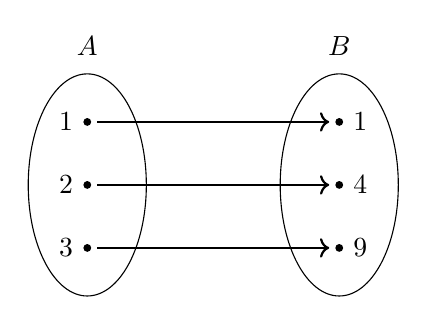
\begin{tikzpicture}[scale=0.8, ele/.style={fill=black,circle,minimum width=.8pt,inner sep=1pt},every fit/.style={ellipse,draw,inner sep=4pt}]
            \node[ele,label=left:$1$] (a1) at (0,3) {};
            \node[ele,label=left:$2$] (a2) at (0,2) {};
            \node[ele,label=left:$3$] (a3) at (0,1) {};

            \node[ele,,label=right:$1$] (b1) at (4,3) {};
            \node[ele,,label=right:$4$] (b2) at (4,2) {};
            \node[ele,,label=right:$9$] (b3) at (4,1) {};

            \node[draw,fit= (a1) (a2) (a3),minimum width=1.5cm] {} ;
            \node[draw,fit= (b1) (b2) (b3),minimum width=1.5cm] {} ;
            \draw[->,thick,shorten <=2pt,shorten >=2] (a1) -- (b1);
            \draw[->,thick,shorten <=2pt,shorten >=2] (a2) -- (b2);
            \draw[->,thick,shorten <=2pt,shorten >=2] (a3) -- (b3);
            \node at (0,4.2) {$A$};
            \node at (4,4.2) {$B$};
          \end{tikzpicture}
        \end{center}
  \item \textbf{Table Method}: express the function in the form of table, showing the relationship of the chosen value between independent variable $x$ and the value of its corresponding dependent variable $y$, as shown below:
        \begin{center}
          \begin{tabular}{|c|c|c|c|}
            \hline
            $x$ & $1$ & $2$ & $3$ \\
            \hline
            $y$ & $1$ & $4$ & $9$ \\
            \hline
          \end{tabular}
        \end{center}

  \item \textbf{Graphical Method}: draw a graph to represent the function of the two variables, as shown below:
        \begin{center}
          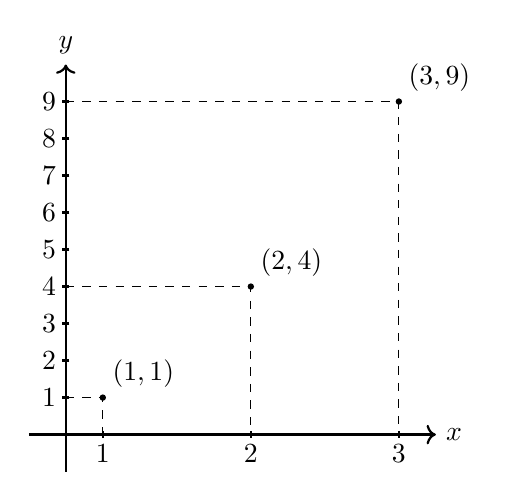
\begin{tikzpicture}[scale=0.47]
            \draw[->,thick] (-1,0) -- (10,0) node[right] {$x$};
            \draw[->,thick] (0,-1) -- (0,10) node[above] {$y$};
            \draw[thick] (1,0.1) -- (1,-0.1);
            \node[below] at (1,0) {1};
            \draw[thick] (5,0.1) -- (5,-0.1);
            \node[below] at (5,0) {2};
            \draw[thick] (9,0.1) -- (9,-0.1);
            \node[below] at (9,0) {3};
            \foreach \y in {1,...,9}
              {
                \draw[thick] (0.1,\y) -- (-0.1,\y);
                \node[left] at (0,\y) {\y};
              }
            \filldraw (1, 1) circle (2pt) node[above right]{$(1,1)$};
            \filldraw (5, 4) circle (2pt) node[above right]{$(2,4)$};
            \filldraw (9, 9) circle (2pt) node[above right]{$(3,9)$};
            \draw[dashed] (0,1) -- (1,1) -- (1,0);
            \draw[dashed] (0,4) -- (5,4) -- (5,0);
            \draw[dashed] (0,9) -- (9,9) -- (9,0);
          \end{tikzpicture}
        \end{center}
\end{enumerate}

\subsection*{Practice 2}

\setlength{\columnseprule}{1pt}
\setlength{\columnsep}{24pt}

\begin{multicols}{2}

  Express the following functions using analytical method, venn diagram, table
  method and graphical method.
  \begin{enumerate}[label=(\alph*)]
    \item $f$ mapping each integers from $-3$ to $3$ to its squares plus $4$.
    \item $g$ mapping each natural numbers from $1$ to $4$ to its cubes.
  \end{enumerate}

\end{multicols}

\subsection*{Exercise 22.1}

\setlength{\columnseprule}{1pt}
\setlength{\columnsep}{24pt}

\begin{multicols}{2}

  \begin{enumerate}
    \item Express the mapping from set $A$ to set $B$, and determine which of the
          following mappings are functions.

          \resizebox{22em}{!}{
            \begin{tabular}{|c|c|c|c|}
              \hline
                  & Set $A$                                & Set $B$                                                                   & Mapping       \\
              \hline
              (a) & \{0, 3, 9, 12\}                        & \{0, 1, 2, 3\}                                                            & Divide by $3$ \\
              \hline
              (b) & \{-2, -1, 0, 1, 2\}                    & \{0, 1, 4, 9, 16\}                                                        & Power of $4$  \\
              \hline
              (c) & \{-2, -1, 0, 1, 2\}                    & \{0, 1, 4\}                                                               & Square        \\
              \hline
              (d) & \{30$^\circ$, 45$^\circ$, 60$^\circ$\} & $\left\{\dfrac{1}{2},\ \dfrac{\sqrt{2}}{2},\ \dfrac{\sqrt{3}}{2}\right\}$ & Sine          \\
              \hline
              (e) & \{-1, 0, 1, 2\}                        & \{-1, 0, 1\}                                                              & Cube          \\
              \hline
            \end{tabular}
          }

    \item Let function $f(x) = 3x^2 + 1$.
          \begin{enumerate}
            \item Find the image of the following elements:
                  \begin{enumerate}
                    \item -3
                    \item -2
                    \item 0
                    \item 2
                    \item 5
                  \end{enumerate}
            \item Find the preimage of the following elements:
                  \begin{enumerate}
                    \item 13
                    \item 28
                    \item 1
                    \item 0
                    \item 4
                  \end{enumerate}
          \end{enumerate}

    \item Let function $g(x) = 5x-2$. Find:
          \begin{enumerate}
            \item $g(-2)$
            \item $g(-1)$
            \item $g(0)$
          \end{enumerate}

    \item Let function $f(x) = \left\{\begin{array}{ll}
              \ \ \ \ \ \ 2x, & x \leq -1     \\
              \ \ x-1,        & -1 \leq x < 3 \\
              4x + 2,         & x \geq 3
            \end{array}\right.$, find

          \begin{enumerate}
            \item $f(-5)$
            \item $f(-2)$
            \item $f(0)$
            \item $f(2)$
            \item $f(10)$
          \end{enumerate}

    \item Let $f: \mathbb{R} \to \mathbb{R}$, $f(x) = x^4$. Find the image of $-1$, 0, 1,
          and 2 under $f$.

    \item Let $f: \mathbb{R} \to \mathbb{R}$, $f(x) = x^4$. Find the preimage of 0, 1,
          and 4 under $f$.

          In $\mathbb{R}$, which element does not have a preimage?

    \item In the diagram below, given that function $g: A \to B$ is defined as $g: x \to
            2x - 8$. Find the value of $a$ and $b$.
          \begin{center}
            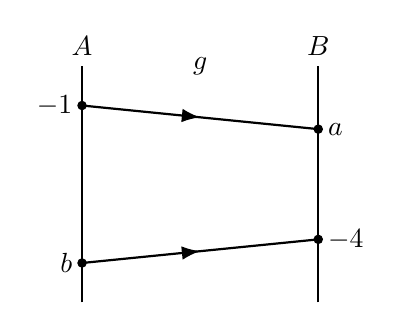
\begin{tikzpicture}
              \draw[thick] (0,0) -- (0,3) node[above]{$A$};
              \draw[thick] (3,0) -- (3,3) node[above]{$B$};
              \node at (1.5, 3) {$g$};
              \filldraw (0, 2.5) circle (1.5pt) node[left]{$-1$};
              \filldraw (0, 0.5) circle (1.5pt) node[left]{$b$};
              \filldraw (3, 0.8) circle (1.5pt) node[right]{$-4$};
              \filldraw (3, 2.2) circle (1.5pt) node[right]{$a$};
              \begin{scope}[thick,decoration={
                      markings,
                      mark=at position 0.5 with {\arrow{Latex}}}
                ]
                \draw[postaction={decorate}] (0, 2.5) -- (3, 2.2);
                \draw[postaction={decorate}] (0, 0.5) -- (3, 0.8);
              \end{scope}
            \end{tikzpicture}
          \end{center}

    \item Using narrative form, arrow method, venn diagram, table method and graphical
          method, express the function $f(x) = 2x$, $x \in \{-2, -1, 0, 1, 2\}$.
  \end{enumerate}
\end{multicols}
\newpage
\section{Domain and Range}

\begin{mdframed}[style=MyFrame]
  Let $f$ is a function from set $A$ to set $B$, then set $A$ is called the domain of $f$, denoted by $D_f$; set $B$ is called the codomain of $f$; the set of the images of all elements of $A$ under $f$ is called the range of $f$, denoted by $R_f$.
\end{mdframed}

If the domain $A$ and range $B$ of function $f: A\to B$ are both subsets of
real number set $\mathbb{R}$, then this function is called real valued function
/ real function. This book primarily discusses about real valued functions.
When the domain of a real function is not mentioned and only the mapping rule
is given, its domain is assumed to be the set of all real numbers that yield
defined values $f(x)$. After the domain and the mapping rule are determined,
the range of a function will then be determined.

\begin{center}
  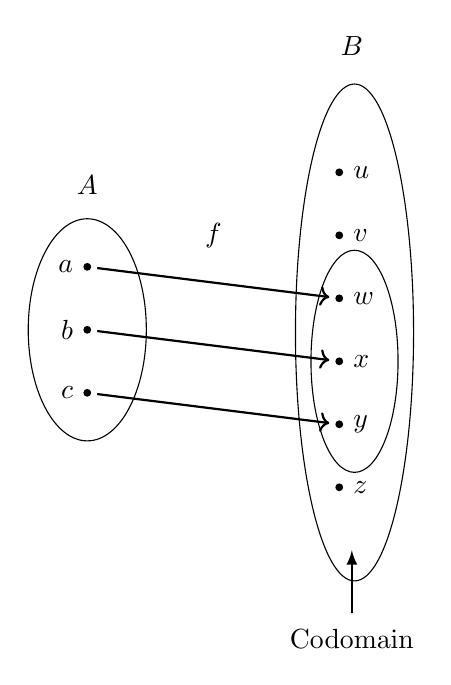
\begin{tikzpicture}[scale=0.8, ele/.style={fill=black,circle,minimum width=.8pt,inner sep=1pt},every fit/.style={ellipse,draw,inner sep=4pt}]
    \node[ele,label=left:$a$] (a1) at (0,4.5) {};
    \node[ele,label=left:$b$] (a2) at (0,3.5) {};
    \node[ele,label=left:$c$] (a3) at (0,2.5) {};

    \node[ele,,label=right:$u$] (b1) at (4,6) {};
    \node[ele,,label=right:$v$] (b2) at (4,5) {};
    \node[ele,,label=right:$w$] (b3) at (4,4) {};
    \node[ele,,label=right:$x$] (b4) at (4,3) {};
    \node[ele,,label=right:$y$] (b5) at (4,2) {};
    \node[ele,,label=right:$z$] (b6) at (4,1) {};
    \node[] (b999) at (4.4,1) {};
    \node[] (b998) at (4.4,3) {};

    \node[draw,fit= (a1) (a2) (a3),minimum width=1.5cm] {} ;
    \node[draw,fit= (b1) (b2) (b3) (b4) (b5) (b6) (b999),minimum width=1.5cm] {} ;
    \node[draw,fit= (b3) (b4) (b5) (b998),minimum width=1cm] {} ;
    \draw[->,thick,shorten <=2pt,shorten >=2] (a1) -- (b3);
    \draw[->,thick,shorten <=2pt,shorten >=2] (a2) -- (b4);
    \draw[->,thick,shorten <=2pt,shorten >=2] (a3) -- (b5);
    \node at (0,5.8) {$A$};
    \node at (4.2,8) {$B$};
    \node at (2,5) {$f$};
    \draw[thick, -latex](4.2,-1) -- (4.2,0);
    \node at (4.2,-1.4) {Codomain};
  \end{tikzpicture}
\end{center}

\begin{mdframed}[style=MyFrame]
  \large{\textbf{Interval Notation}}
  \normalsize

  \noindent Let $a$ and $b$ be two real number, $a < b$.
  \begin{center}
    \begin{tabular}{|c|c|}
      \hline
      Intervals      & Set Notations                                          \\
      \hline
      $(a, b)$       & $\left\{x | x \in \mathbb{R}, a < x < b\right\}$       \\
      $[a, b)$       & $\left\{x | x \in \mathbb{R}, a \leq x < b\right\}$    \\
      $(a, b]$       & $\left\{x | x \in \mathbb{R}, a < x \leq b\right\}$    \\
      $[a, b]$       & $\left\{x | x \in \mathbb{R}, a \leq x \leq b\right\}$ \\
      $(a, \infty)$  & $\left\{x | x \in \mathbb{R}, x > a\right\}$           \\
      $[a, \infty)$  & $\left\{x | x \in \mathbb{R}, x \leq a\right\}$        \\
      $(-\infty, a)$ & $\left\{x | x \in \mathbb{R}, x < a\right\}$           \\
      $(-\infty, a]$ & $\left\{x | x \in \mathbb{R}, x \leq a\right\}$        \\
      \hline
    \end{tabular}
  \end{center}
\end{mdframed}

\subsection*{Practice 3}

\setlength{\columnseprule}{1pt}
\setlength{\columnsep}{24pt}

\begin{multicols}{2}

  \begin{enumerate}
    \item Let $A = \{2, 4, 5, 7\}$ and $B = \{3, 5, 7, 8, 9\}$, the definition of
          function $g$ is given by the diagram below. Find the domain, codomain and range
          of function $g$.
          \begin{center}
            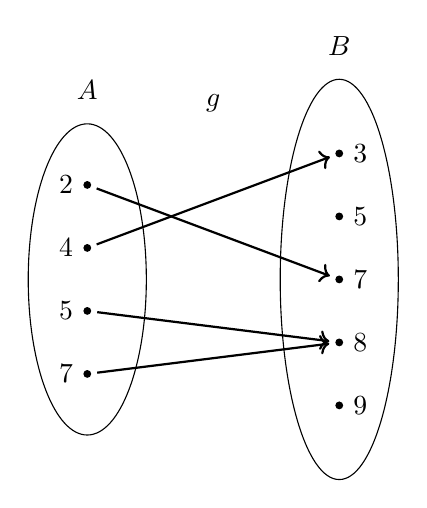
\begin{tikzpicture}[scale=0.8, ele/.style={fill=black,circle,minimum width=.8pt,inner sep=1pt},every fit/.style={ellipse,draw,inner sep=4pt}]
              \node[ele,label=left:$2$] (a1) at (0,3.5) {};
              \node[ele,label=left:$4$] (a2) at (0,2.5) {};
              \node[ele,label=left:$5$] (a3) at (0,1.5) {};
              \node[ele,label=left:$7$] (a4) at (0,0.5) {};

              \node[ele,,label=right:$3$] (b1) at (4,4) {};
              \node[ele,,label=right:$5$] (b2) at (4,3) {};
              \node[ele,,label=right:$7$] (b3) at (4,2) {};
              \node[ele,,label=right:$8$] (b4) at (4,1) {};
              \node[ele,,label=right:$9$] (b5) at (4,0) {};

              \node[draw,fit= (a1) (a2) (a3) (a4),minimum width=1.5cm] {} ;
              \node[draw,fit= (b1) (b2) (b3) (b4) (b5),minimum width=1.5cm] {} ;
              \draw[->,thick,shorten <=2pt,shorten >=2] (a1) -- (b3);
              \draw[->,thick,shorten <=2pt,shorten >=2] (a2) -- (b1);
              \draw[->,thick,shorten <=2pt,shorten >=2] (a3) -- (b4);
              \draw[->,thick,shorten <=2pt,shorten >=2] (a4) -- (b4);
              \node at (0,5) {$A$};
              \node at (4,5.7) {$B$};
              \node at (2,4.8) {$g$};
            \end{tikzpicture}
          \end{center}

    \item Let $A = \{-2, -1, 0, 1, 2\}$, function $f: A \to \mathbb{R}$ is defined by
          $f(x) = x^2 - 1$. Find the domain and range of $f$.

    \item The curve in the diagram below represents the function $y = f(x)$, $-2 \leq x
            \leq 3$. Find the domain and range of $f$.
          \begin{center}
            \begin{tikzpicture}
              \begin{axis}[
                  axis lines=middle,
                  xmin=-2.5, xmax=3.5,
                  ymin=-3, ymax=8,
                  xtick={-2,-1,0,1,2,3},
                  ytick={-2, -1, ..., 7},
                  xlabel={$x$},
                  ylabel={$y$},
                  xlabel style={anchor=east, xshift=0.5cm},
                  ylabel style={anchor=north, yshift=0.5cm},
                  xtick style={thick, color=black},
                  ytick style={thick, color=black},
                  line style={thick, color=black},
                ]
                \addplot[domain=-2:3, thick] {x^2 - 2};
                \path (axis cs:0,0)
                node [anchor=north east, xshift=0.05cm] {0};
                \draw[dashed] (axis cs:0,7) -- (axis cs:3,7);
                \filldraw (axis cs:3,7) circle (1.6pt);
                \draw[dashed] (axis cs:0,2) -- (axis cs:-2,2);
                \filldraw (axis cs:-2,2) circle (1.6pt);
              \end{axis}
            \end{tikzpicture}
          \end{center}

    \item Find the domain and range of the following functions:
          \begin{enumerate}
            \item $f(x) = -4x + 5$
            \item $g(x) = x^2 - 1$
            \item $h(x) = \dfrac{1}{4x + 7}$
            \item $k(x) = \sqrt{6 - x}$
          \end{enumerate}
  \end{enumerate}

\end{multicols}

\subsection*{Exercise 22.2}

\setlength{\columnseprule}{1pt}
\setlength{\columnsep}{24pt}

\begin{multicols}{2}

  \begin{enumerate}
    \item Let $X = \{a, b, c, d\}$ and $Y = \{-1, 2, 9, 11\}$, function $f: X \to Y$ is
          defined by $f(a) = 2$, $f(b) = -1$, $f(c) = 2$, $f(d) = 9$. Find the domain and
          range of the $f$.

    \item The curve in the diagram below represents the function $y = f(x)$, $-1 < x \leq
            4$. Find the domain and range of $f$.
          \begin{center}
            \begin{tikzpicture}
              \begin{axis}[
                  axis lines=middle,
                  xmin=-2.5, xmax=4.5,
                  ymin=-4, ymax=8,
                  xtick={-2,-1,0,1,2,3,4},
                  ytick={-3, -2, -1, ..., 7},
                  xlabel={$x$},
                  ylabel={$y$},
                  xlabel style={anchor=east, xshift=0.5cm},
                  ylabel style={anchor=north, yshift=0.5cm},
                  xtick style={thick, color=black},
                  ytick style={thick, color=black},
                  line style={thick, color=black},
                ]
                \addplot[domain=-1:4, thick] {-(x - 1)^2 + 6};
                \path (axis cs:0,0)
                node [anchor=north east, xshift=0.05cm] {0};
                \draw[dashed] (axis cs:0,-3) -- (axis cs:4,-3);
                \filldraw (axis cs:4,-3) circle (1.6pt);
                \draw[dashed] (axis cs:0,2) -- (axis cs:-1,2);
                \filldraw[fill=white] (axis cs:-1,2) circle (1.6pt);
              \end{axis}
            \end{tikzpicture}
          \end{center}

    \item Let $A = \{a, b, c, d, e\}$ and $B = \{4, 5, 8, 9, 12\}$, the definition of
          function $g: A \to B$ is given by the digram below. Find the domain, codomain
          and range of function $g$.
          \begin{center}
            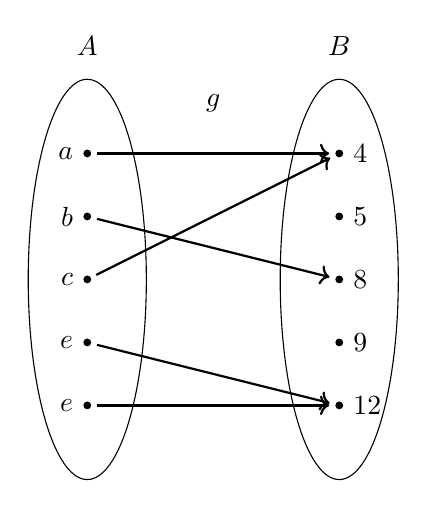
\begin{tikzpicture}[scale=0.8, ele/.style={fill=black,circle,minimum width=.8pt,inner sep=1pt},every fit/.style={ellipse,draw,inner sep=4pt}]
              \node[ele,label=left:$a$] (a1) at (0,4) {};
              \node[ele,label=left:$b$] (a2) at (0,3) {};
              \node[ele,label=left:$c$] (a3) at (0,2) {};
              \node[ele,label=left:$e$] (a4) at (0,1) {};
              \node[ele,label=left:$e$] (a5) at (0,0) {};

              \node[ele,,label=right:$4$] (b1) at (4,4) {};
              \node[ele,,label=right:$5$] (b2) at (4,3) {};
              \node[ele,,label=right:$8$] (b3) at (4,2) {};
              \node[ele,,label=right:$9$] (b4) at (4,1) {};
              \node[ele,,label=right:$12$] (b5) at (4,0) {};

              \node[draw,fit= (a1) (a2) (a3) (a4) (a5),minimum width=1.5cm] {} ;
              \node[draw,fit= (b1) (b2) (b3) (b4) (b5),minimum width=1.5cm] {} ;
              \draw[->,thick,shorten <=2pt,shorten >=2] (a1) -- (b1);
              \draw[->,thick,shorten <=2pt,shorten >=2] (a2) -- (b3);
              \draw[->,thick,shorten <=2pt,shorten >=2] (a3) -- (b1);
              \draw[->,thick,shorten <=2pt,shorten >=2] (a4) -- (b5);
              \draw[->,thick,shorten <=2pt,shorten >=2] (a5) -- (b5);
              \node at (0,5.7) {$A$};
              \node at (4,5.7) {$B$};
              \node at (2,4.8) {$g$};
            \end{tikzpicture}
          \end{center}

    \item Let $A = \{-1, 0, 1, 2\}$, function $f: A \to \mathbb{R}$ is defined by $f(x) =
            3x^2 - 2$, find the domain and range of $f$.

    \item Let $A = \{-1, 0, 2, 5, 11\}$, function $f: A \to \mathbb{R}$ is defined by
          $f(x) = x^2 - x - 2$, find the domain and range of $f$.

    \item Find the domain and range of the following functions:
          \begin{enumerate}
            \item $f(x) = x^3$
            \item $g(x) = \sqrt{1 - x^2}$
            \item $h(x) = \dfrac{1}{2x + 3}$
            \item $k(x) = x^2 - 2x + 4$
          \end{enumerate}
  \end{enumerate}

\end{multicols}

\newpage
\section{Graphs of Functions and Their Transformations}
\subsection*{Graphs of Simple Functions}

On a Cartesian plane, the graphs formed by all the point $(x, y)$ that
satisfied the equation $y = f(x)$ are called graphs of function $f$. Below are
some examples of graphs of simple functions.

Note that any line that is parallel to the $y$-axis intersects the graph of a
function at most once. \setlength{\columnseprule}{0pt}
\setlength{\columnsep}{24pt}

\begin{multicols}{2}
  \begin{enumerate}[label=(\alph*)]
    \item $y = x$
          \begin{center}
            \resizebox{0.33\textwidth}{!}{
              \begin{tikzpicture}
                \begin{axis}[
                    axis lines=middle,
                    xmin=-5.5, xmax=5.5,
                    ymin=-5.5, ymax=5.5,
                    xlabel={$x$},
                    ylabel={$y$},
                    ticks=none,
                    xlabel style={anchor=east, xshift=0.5cm},
                    ylabel style={anchor=north, yshift=0.5cm},
                    line style={thick, color=black},
                  ]
                  \addplot[domain=-5:5, thick] {x};
                  \path (axis cs:0,0)
                  node [anchor=north east, xshift=0.05cm] {$O$};
                \end{axis}
              \end{tikzpicture}
            }
          \end{center}

    \item $y = -x$
          \begin{center}
            \resizebox{0.33\textwidth}{!}{
              \begin{tikzpicture}
                \begin{axis}[
                    axis lines=middle,
                    xmin=-5.5, xmax=5.5,
                    ymin=-5.5, ymax=5.5,
                    xlabel={$x$},
                    ylabel={$y$},
                    ticks=none,
                    xlabel style={anchor=east, xshift=0.5cm},
                    ylabel style={anchor=north, yshift=0.5cm},
                    line style={thick, color=black},
                  ]
                  \addplot[domain=-5:5, thick] {-x};
                  \path (axis cs:0,0)
                  node [anchor=north east, xshift=0.05cm] {$O$};
                \end{axis}
              \end{tikzpicture}
            }
          \end{center}
  \end{enumerate}
\end{multicols}
\begin{multicols}{2}
  \begin{enumerate}[label=(\alph*)]
    \setcounter{enumi}{2}
    \item $y = x^2$
          \begin{center}
            \resizebox{0.33\textwidth}{!}{
              \begin{tikzpicture}
                \begin{axis}[
                    axis lines=middle,
                    xmin=-2.5, xmax=2.5,
                    ymin=-0.5, ymax=5.5,
                    xlabel={$x$},
                    ylabel={$y$},
                    ticks=none,
                    xlabel style={anchor=east, xshift=0.5cm},
                    ylabel style={anchor=north, yshift=0.5cm},
                    line style={thick, color=black},
                  ]
                  \addplot[domain=-5:5, thick] {x^2};
                  \path (axis cs:0,0)
                  node [anchor=north east, xshift=0.05cm] {$O$};
                \end{axis}
              \end{tikzpicture}
            }
          \end{center}

    \item $y = x^2$
          \begin{center}
            \resizebox{0.33\textwidth}{!}{
              \begin{tikzpicture}
                \begin{axis}[
                    axis lines=middle,
                    xmin=-2.5, xmax=2.5,
                    ymin=-5.5, ymax=0.5,
                    xlabel={$x$},
                    ylabel={$y$},
                    ticks=none,
                    xlabel style={anchor=east, xshift=0.5cm},
                    ylabel style={anchor=north, yshift=0.5cm},
                    line style={thick, color=black},
                  ]
                  \addplot[domain=-5:5, thick] {-x^2};
                  \path (axis cs:0,0)
                  node [anchor=north east, xshift=0.05cm] {$O$};
                \end{axis}
              \end{tikzpicture}
            }
          \end{center}
  \end{enumerate}
\end{multicols}
\begin{multicols}{2}
  \begin{enumerate}[label=(\alph*)]
    \setcounter{enumi}{4}
    \item $y = x^3$
          \begin{center}
            \resizebox{0.33\textwidth}{!}{
              \begin{tikzpicture}
                \begin{axis}[
                    axis lines=middle,
                    xmin=-2.5, xmax=2.5,
                    ymin=-5.5, ymax=5.5,
                    xlabel={$x$},
                    ylabel={$y$},
                    ticks=none,
                    xlabel style={anchor=east, xshift=0.5cm},
                    ylabel style={anchor=north, yshift=0.5cm},
                    line style={thick, color=black},
                  ]
                  \addplot[domain=-5:5, thick] {x^3};
                  \path (axis cs:0,0)
                  node [anchor=north east, xshift=0.05cm] {$O$};
                \end{axis}
              \end{tikzpicture}
            }
          \end{center}

    \item $y = -x^3$
          \begin{center}
            \resizebox{0.33\textwidth}{!}{
              \begin{tikzpicture}
                \begin{axis}[
                    axis lines=middle,
                    xmin=-2.5, xmax=2.5,
                    ymin=-5.5, ymax=5.5,
                    xlabel={$x$},
                    ylabel={$y$},
                    ticks=none,
                    xlabel style={anchor=east, xshift=0.5cm},
                    ylabel style={anchor=north, yshift=0.5cm},
                    line style={thick, color=black},
                  ]
                  \addplot[domain=-5:5, thick] {-x^3};
                  \path (axis cs:0,0)
                  node [anchor=north east, xshift=0.05cm] {$O$};
                \end{axis}
              \end{tikzpicture}
            }
          \end{center}
  \end{enumerate}
\end{multicols}
\newpage
\begin{multicols}{2}
  \begin{enumerate}[label=(\alph*)]
    \setcounter{enumi}{6}
    \item $y = \dfrac{1}{x}$
          \begin{center}
            \resizebox{0.33\textwidth}{!}{
              \begin{tikzpicture}
                \begin{axis}[
                    axis lines=middle,
                    xmin=-5.5, xmax=5.5,
                    ymin=-5.5, ymax=5.5,
                    xlabel={$x$},
                    ylabel={$y$},
                    ticks=none,
                    xlabel style={anchor=east, xshift=0.5cm},
                    ylabel style={anchor=north, yshift=0.5cm},
                    line style={thick, color=black},
                  ]
                  \addplot[domain=-5:-0.01, thick] {1/x};
                  \addplot[domain=0.01:5, thick] {1/x};
                  \path (axis cs:0,0)
                  node [anchor=north east, xshift=0.05cm] {$O$};
                \end{axis}
              \end{tikzpicture}
            }
          \end{center}

    \item $y = -\dfrac{1}{x}$
          \begin{center}
            \resizebox{0.33\textwidth}{!}{
              \begin{tikzpicture}
                \begin{axis}[
                    axis lines=middle,
                    xmin=-5.5, xmax=5.5,
                    ymin=-5.5, ymax=5.5,
                    xlabel={$x$},
                    ylabel={$y$},
                    ticks=none,
                    xlabel style={anchor=east, xshift=0.5cm},
                    ylabel style={anchor=north, yshift=0.5cm},
                    line style={thick, color=black},
                  ]
                  \addplot[domain=-5:-0.01, thick] {-1/x};
                  \addplot[domain=0.01:5, thick] {-1/x};
                  \path (axis cs:0,0)
                  node [anchor=north east, xshift=0.05cm] {$O$};
                \end{axis}
              \end{tikzpicture}
            }
          \end{center}
  \end{enumerate}
\end{multicols}
\begin{multicols}{2}
  \begin{enumerate}[label=(\alph*)]
    \setcounter{enumi}{8}
    \item $y = \dfrac{1}{x^2}$
          \begin{center}
            \resizebox{0.33\textwidth}{!}{
              \begin{tikzpicture}
                \begin{axis}[
                    axis lines=middle,
                    xmin=-5.5, xmax=5.5,
                    ymin=-0.5, ymax=5.5,
                    xlabel={$x$},
                    ylabel={$y$},
                    ticks=none,
                    xlabel style={anchor=east, xshift=0.5cm},
                    ylabel style={anchor=north, yshift=0.5cm},
                    line style={thick, color=black},
                  ]
                  \addplot[domain=-5:-0.05, thick] {1/x^2};
                  \addplot[domain=0.05:5, thick] {1/x^2};
                  \path (axis cs:0,0)
                  node [anchor=north east, xshift=0.05cm] {$O$};
                \end{axis}
              \end{tikzpicture}
            }
          \end{center}

    \item $y = -\dfrac{1}{x^2}$
          \begin{center}
            \resizebox{0.33\textwidth}{!}{
              \begin{tikzpicture}
                \begin{axis}[
                    axis lines=middle,
                    xmin=-5.5, xmax=5.5,
                    ymin=-5.5, ymax=0.5,
                    xlabel={$x$},
                    ylabel={$y$},
                    ticks=none,
                    xlabel style={anchor=east, xshift=0.5cm},
                    ylabel style={anchor=north, yshift=0.5cm},
                    line style={thick, color=black},
                  ]
                  \addplot[domain=-5:-0.05, thick] {-1/x^2};
                  \addplot[domain=0.05:5, thick] {-1/x^2};
                  \path (axis cs:0,0)
                  node [anchor=north east, xshift=0.05cm] {$O$};
                \end{axis}
              \end{tikzpicture}
            }
          \end{center}
  \end{enumerate}
\end{multicols}
\begin{multicols}{2}
  \begin{enumerate}[label=(\alph*)]
    \setcounter{enumi}{10}
    \item $y = \sqrt{x}$
          \begin{center}
            \resizebox{0.33\textwidth}{!}{
              \begin{tikzpicture}
                \begin{axis}[
                    axis lines=middle,
                    xmin=-0.5, xmax=3.5,
                    ymin=-0.5, ymax=3.5,
                    xlabel={$x$},
                    ylabel={$y$},
                    ticks=none,
                    xlabel style={anchor=east, xshift=0.5cm},
                    ylabel style={anchor=north, yshift=0.5cm},
                    line style={thick, color=black},
                  ]
                  \addplot[domain=0:5, thick] {x^0.5};
                  \path (axis cs:0,0)
                  node [anchor=north east, xshift=0.05cm] {$O$};
                \end{axis}
              \end{tikzpicture}
            }
          \end{center}

    \item $y = -\sqrt{x}$
          \begin{center}
            \resizebox{0.33\textwidth}{!}{
              \begin{tikzpicture}
                \begin{axis}[
                    axis lines=middle,
                    xmin=-0.5, xmax=3.5,
                    ymin=-3.5, ymax=0.5,
                    xlabel={$x$},
                    ylabel={$y$},
                    ticks=none,
                    xlabel style={anchor=east, xshift=0.5cm},
                    ylabel style={anchor=north, yshift=0.5cm},
                    line style={thick, color=black},
                  ]
                  \addplot[domain=0:5, thick] {-x^0.5};
                  \path (axis cs:0,0)
                  node [anchor=north east, xshift=0.05cm] {$O$};
                \end{axis}
              \end{tikzpicture}
            }
          \end{center}
  \end{enumerate}
\end{multicols}
\subsection*{Transformations of Graphs}

\begin{mdframed}[style=MyFrame]
  \begin{itemize}[leftmargin=0.3cm]
    \item If $k > 0$, translate the graph of $y = f(x)$ vertically upwards by $k$ units,
          the graph of $y = f(x) + k$ is obtained.

    \item If $k > 0$, translate the graph of $y = f(x)$ vertically downwards by $k$
          units, the graph of $y = f(x) - k$ is obtained.
  \end{itemize}
\end{mdframed}

\begin{center}
  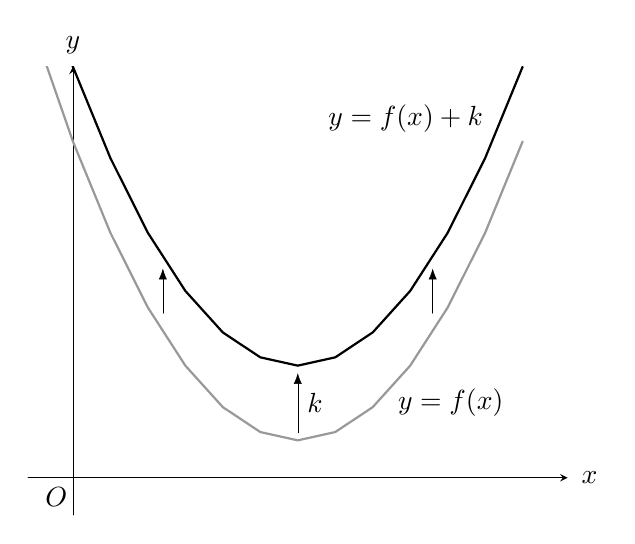
\begin{tikzpicture}
    \begin{axis}[
        axis lines=middle,
        xmin=-0.5, xmax=5.5,
        ymin=-0.5, ymax=5.5,
        xlabel={$x$},
        ylabel={$y$},
        ticks=none,
        xlabel style={anchor=east, xshift=0.5cm},
        ylabel style={anchor=north, yshift=0.5cm},
        line style={thick, color=black},
      ]
      \addplot[domain=-5:5, thick, color=black!40] {(0.8*x-2)^2 + 0.5};
      \addplot[domain=-5:5, thick] {(0.8*x-2)^2 + 1.5};
      \path (axis cs:0,0)
      node [anchor=north east, xshift=0.05cm] {$O$};
      \draw[-Latex] (axis cs:2.5, 0.6) -- (axis cs:2.5, 1.4) node [midway, right] {$k$};
      \draw[-Latex] (axis cs:1, 2.2) -- (axis cs:1, 2.8);
      \draw[-Latex] (axis cs:4, 2.2) -- (axis cs:4, 2.8);
      \node at (axis cs:3.7, 4.8) {$y = f(x) + k$};
      \node at (axis cs:4.2, 1) {$y = f(x)$};
    \end{axis}
  \end{tikzpicture}
  \hspace{1cm}
  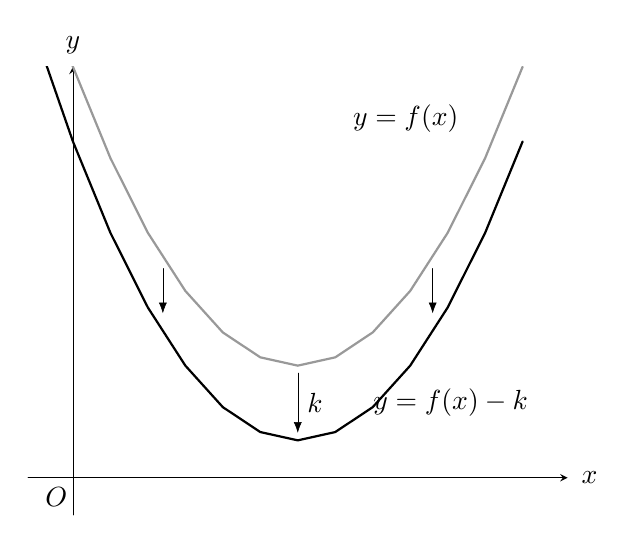
\begin{tikzpicture}
    \begin{axis}[
        axis lines=middle,
        xmin=-0.5, xmax=5.5,
        ymin=-0.5, ymax=5.5,
        xlabel={$x$},
        ylabel={$y$},
        ticks=none,
        xlabel style={anchor=east, xshift=0.5cm},
        ylabel style={anchor=north, yshift=0.5cm},
        line style={thick, color=black},
      ]
      \addplot[domain=-5:5, thick] {(0.8*x-2)^2 + 0.5};
      \addplot[domain=-5:5, thick, color=black!40] {(0.8*x-2)^2 + 1.5};
      \path (axis cs:0,0)
      node [anchor=north east, xshift=0.05cm] {$O$};
      \draw[-Latex] (axis cs:2.5, 1.4) -- (axis cs:2.5, 0.6) node [midway, right] {$k$};
      \draw[-Latex] (axis cs:1, 2.8) -- (axis cs:1, 2.2);
      \draw[-Latex] (axis cs:4, 2.8) -- (axis cs:4, 2.2);
      \node at (axis cs:3.7, 4.8) {$y = f(x)$};
      \node at (axis cs:4.2, 1) {$y = f(x) - k$};
    \end{axis}
  \end{tikzpicture}

\end{center}

\begin{mdframed}[style=MyFrame]
  \begin{itemize}[leftmargin=0.3cm]
    \item If $h > 0$, translate the graph of $y = f(x)$ horizontally to the right by $h$
          units, the graph of $y = f(x + h)$ is obtained.

    \item If $h > 0$, translate the graph of $y = f(x)$ horizontally to the left by $h$
          units, the graph of $y = f(x - h)$ is obtained.
  \end{itemize}
\end{mdframed}

\begin{mdframed}[style=MyFrame]
  \begin{itemize}[leftmargin=0.3cm]
    \item If $k > 0$, reflect the graph of $y = f(x)$ about the $x$-axis, the graph of $y
            = -f(x)$ is obtained.

    \item If $k > 0$, reflect the graph of $y = f(x)$ about the $y$-axis, the graph of $y
            = f(-x)$ is obtained.
  \end{itemize}
\end{mdframed}

\begin{mdframed}[style=MyFrame]
  If $a > 0$, zooming (when $a > 1$) or shrinking (when $0 < a < 1$) the graph of $y = f(x)$ by a factor of $a$ in the $y$-direction, the graph of $y = af(x)$ is obtained.
\end{mdframed}

\begin{mdframed}[style=MyFrame]
  If $a > 0$, shrinking (when $a > 1$) or zooming (when $0 < a < 1$) the graph of $y = f(x)$ by a factor of $\dfrac{1}{a}$ in the $x$-direction, the graph of $y = f(ax)$ is obtained.
\end{mdframed}

\subsection*{Practice 4}

\setlength{\columnseprule}{1pt}
\setlength{\columnsep}{24pt}

\begin{multicols}{2}

  Find the line of symmetry and vertex of the following parabola, and sketch its
  graph. (Question 1 to 2):
  \begin{enumerate}
    \item $y = 2x^2 + 8x + 11$
    \item $y = -3x^2 + 18x - 7$
  \end{enumerate}

  Sketch the graph of the following functions. (Question 3 to 4):
  \begin{enumerate}
    \setcounter{enumi}{2}
    \item $y = \dfrac{4}{{(x+2)}^2}$
    \item $y = \sqrt{x - 1} + 3$
  \end{enumerate}

\end{multicols}

\setlength{\columnseprule}{1pt}
\setlength{\columnsep}{24pt}

\subsection*{Exercise 22.3}

\begin{multicols}{2}

  Find the line of symmetry and vertex of the following parabola, and sketch its
  graph.
  \begin{enumerate}
    \item $y = 2x^2 + 4x + 5$
    \item $y = -3x^2 + 12x - 4$
    \item $y = 4x^2 - 20x + 19$
    \item $y = -3x^2 - 6x - 4$
  \end{enumerate}

  Sketch the graph of the following functions.
  \begin{enumerate}
    \setcounter{enumi}{4}
    \item $y = (x+2)^3 - 5$
    \item $y = \sqrt{x-5}$
    \item $y = \dfrac{1}{(x+2)^2}$
    \item $y = -\dfrac{1}{2(x-1)^2}$
    \item $y = 3\sqrt{x+1} - 4$
    \item $y = \dfrac{4}{2x+3}$
    \item $y = \left\{\begin{array}{ll}
              4x+9,   & x \leq 0 \\
              9 - 2x, & x > 0    \\
            \end{array}\right.$
    \item $y = \left\{\begin{array}{ll}
              \ \ \ \ \ \ \ \ \ \ x, & x < -1    \\
              \sqrt{x+1},            & x \geq -1 \\
            \end{array}\right.$
  \end{enumerate}

  \begin{enumerate}
    \setcounter{enumi}{12}
    \item Sketch the graph for the function $f(x) = x^2 - 6x + 12$, $-2 \leq x \leq 8$,
          and find its domain and range.
    \item Sketch the graph for the function $g(x) = -x^2 - 4x - 7$, $-2 \leq x \leq 5$,
          and find its domain and range.
    \item Sketch the graph for the function $f(x) = -x^2 + 2x + 10$, and find its domain
          and range.
    \item Sketch the graph of the function $y = \sqrt{x}$, and transform it according the
          following steps. Sketch the graph of each function after each step on the same
          diagram, and write down the corresponding function.

          Step 1: Translate 4 units to the left;

          Step 2: Scale up by a factor of 2 in the $x$-direction;

          Step 3: Reflect about the $y$-axis;

          Step 4: Translate 3 units downwards.

          Step 5: Scale down by half in the $y$-direction.
  \end{enumerate}

\end{multicols}

\section{Composite Functions}

Let $A$, $B$, and $C$ be three non-empty sets, $f: A \to B$ and $g: B \to C$ be
two functions, an element $x$ in set $A$ is mapped to an element $f(x)$ in set
$B$ by function $f$, and $f(x)$ is mapped to an element $g\big(f(x)\big)$ in
set $C$ by function $g$. In other words, $x$ in set $A$ is mapped to an element
$g\big(f(x)\big)$ in $C$ after two mappings. That is:
\begin{cequation}
  x\ \xrightarrow{\displaystyle \ \ f\ \ } f(x)\ \xrightarrow{\displaystyle \ \ g\ \ } g\big(f(x)\big)
\end{cequation}

The combination of these two mappings are a function from set $A$ to set $C$,
this function is called the \emph{composite function} of $f$ and $g$, denoted
by $g \circ f$. When defining the composite function $g \circ f$, the range of
$f$ must be a subset of the domain of $g$, that is, $R_f \subseteq D_g$.

Note that $D_{g \circ f} = D_f$, $R_{g \circ f} \subseteq R_g$.

$\forall n \in \mathbb{N}$, $f^{n+1} = f \circ f^n$.

Generally speaking, $g \circ f \neq f \circ g$.

If $f \circ (g \circ h)$ is defined, then $(f \circ g) \circ h$ is also
defined, and $f \circ (g \circ h) = (f \circ g) \circ h$. Therefore, we can
write $f \circ g \circ h$ without ambiguity.

\subsection*{Practice 5}

\setlength{\columnseprule}{1pt}
\setlength{\columnsep}{24pt}

\begin{multicols}{2}

  \begin{enumerate}[label=\arabic*., leftmargin=*]
    \item Let $f: \mathbb{R} \to \mathbb{R}$, $f(x) = 2x + 3$ and $g: \mathbb{R} \to
            \mathbb{R}$, $g(x) = 5 - x$. Find $(g \circ f)(x)$ and $(f \circ g)(x)$.

    \item Let $f: \mathbb{R} \to \mathbb{R}$, $f(x) = x^2 - 2x + 3$ and $g: \mathbb{R}
            \to \mathbb{R}$, $g(x) = 3x - 4$. Find
          \begin{enumerate}
            \item $g \circ f$ and $f \circ g$;
            \item $g\big(f(2)\big)$, $f\big(g(2)\big)$, $(g \circ f)(2)$, and $(f \circ g)(2)$.
          \end{enumerate}

    \item Let $f: \mathbb{R} \to \mathbb{R}$, $f(x) = 4 - x^2$ and $g: \left\{x | x \leq
            4 \right\} \to \mathbb{R}$, $g(x) = \sqrt{4 - x}$. Prove the existence of $f
            \circ g$ and $g \circ f$ respectively.
  \end{enumerate}

\end{multicols}

\section{One to One Function, Onto Function and One to One Onto Function}

\subsection*{One to One Function}

Let $f: A \to B$ be a function, if there is at most one preimage in set $A$ for
each element in set $B$, then $f$ is called a \emph{one to one function}.

As shown in the diagram above, each element in the codomain $B$ of the function
$f: A \to B$ has at most one preimage in the domain $A$ of the function, thus
$f$ is a one to one function; while the element $b_2$ in the codomain $B$ of
the function $g: A \to B$ has two preimages $a_2$ and $a_3$, thus $g$ is not a
one to one function.

A function $y = f(x)$ is a one to one function, if and only if any line
parallel to the $x$-axis intersects the graph of the function at most once.

\subsection*{Onto Function}

If each element in the codomain $B$ of the function $f: A \to B$ has at least
one preimage under the function $f$, then $f$ is said to be an \emph{onto
  function}.

As shown in the diagram above, each element in the codomain $B$ of the function
$f: A \to B$ has at least one preimage under the function $f$, therefore $f$ is
an onto function; while the element $b_3$ in the codomain $B$ of the function
$g: A \to B$ has no preimage under the function $g$, therefore $g$ is not an
onto function.

\subsection*{One to One Onto Function}

If a function is both a one to one function and an onto function, then it is a
\emph{one to one onto function}, as shown in the diagram above.

\subsection*{Practice 7}

Determine whether the following functions are one to one functions or onto
functions.

\subsection*{Exercise 22.5}

\setlength{\columnseprule}{1pt}
\setlength{\columnsep}{24pt}

\begin{multicols}{2}

  \begin{enumerate}
    \item Let $A = \left\{1, 2, 3\right\}$, $f: A \to A$ is defined by $f: 1 \to 1$, $2
            \to 3$, $3 \to 2$. Determine if $f$ is a one to one function or an onto
          function.

    \item Let $A = \left\{a, b, c, d\right\}$ and $B = \left\{x, y, z\right\}$, $f: A \to
            B$ is defined by $f: a \to y$, $b \to x$, $c \to z$, $d \to y$. Determine if
          $f$ is a one to one function or an onto function.

    \item Let the function $g: \mathbb{R} \to \mathbb{R}$ be defined by $g(x) = 2x + 1$.
          Determine if $g$ is a one to one function or an onto function.

    \item Let the function $f: \mathbb{R} \to \mathbb{R}$ be defined by $f(x) = 2x^3 -
            3$. Determine if $f$ is a one to one function or an onto function.

    \item Let the function $f: \mathbb{R}^+ \to \mathbb{R}^+$ be defined by $f(x) =
            \dfrac{1}{x}$. Determine if $f$ is a one to one function or an onto function.

    \item Let the function $f: \mathbb{R}^+ \to \mathbb{R}^+$ be defined by $f(x) =
            \sqrt{x}$. Determine if $f$ is a one to one function or an onto function.

    \item Determine whether the following functions are one to one, onto or one to one
          onto functions.
          \begin{enumerate}
            \item $A = \left\{a, b, c\right\}$, $B = \left\{x, y, z\right\}$, $f: A \to
                    B$, $f: a \to x$, $b \to x$, $c \to y$
            \item $A = \left\{a, b, c\right\}$, $B = \left\{x, y, z\right\}$, $g: A \to
                    B$, $g: a \to x$, $b \to y$, $c \to z$
            \item $A = \left\{a, b, c\right\}$, $B = \left\{x, y\right\}$, $h: A \to
                    B$, $h: a \to x$, $b \to y$, $c \to y$
            \item $A = \left\{a, b, c\right\}$, $B = \left\{x, y\right\}$, $k: A \to
                    B$, $k: a \to x$, $a \to y$, $c \to y$
            \item $A = \left\{a, b, c\right\}$, $B = \left\{x, y\right\}$, $f: A \to B$, $f: a \to x$, $a \to y$, $b \to x$, $c \to y$
            \item $A = \left\{a, b, c, d\right\}$, $B = \left\{u, v, x, y, z\right\}$, $g: A \to B$, $g: a \to u$, $b \to v$, $c \to x$, $d \to y$
          \end{enumerate}

    \item Determine whether the following functions mapping $A$ to $B$ are one to one
          functions or onto functions.
  \end{enumerate}

\end{multicols}

\newpage

\section{Inverse Functions}

\begin{mdframed}[style=MyFrame]
  If $f: A \to B$ is a one to one onto function, then there exist a function $g: B \to A$, such that if $y = f(x)$, then $g(y) = x$. The function $g$ is called the \emph{inverse function} of $f$, and is denoted by $f^{-1}$.
\end{mdframed}

from the diagram above, we can conclude the following:

\begin{mdframed}[style=MyFrame]
  \begin{cequation}
    x\ \xrightarrow{\displaystyle \ \ f\ \ } y = f(x)\ \xrightarrow{\displaystyle \ \ f^{-1}\ \ } f^{-1}\big(f(x)\big) = f^{-1}(y)
  \end{cequation}
\end{mdframed}
or
\begin{mdframed}[style=MyFrame]
  \begin{cequation}
    y\ \xrightarrow{\displaystyle \ \ f^{-1}\ \ } x = f^{-1}(y)\ \xrightarrow{\displaystyle \ \ f\ \ } f\big(f^{-1}(y)\big) = f(x)
  \end{cequation}
\end{mdframed}

If both $(g\circ f)^-1$ and $f^{-1} \circ g^{-1}$ exist, then $(g\circ f)^{-1}
  = f^{-1} \circ g^{-1}$.

\subsection*{Practice 8}

\subsection*{Exercise 22.5}

\setlength{\columnseprule}{1pt}
\setlength{\columnsep}{24pt}

\begin{multicols}{2}

  \begin{enumerate}
    \item Find the inverse function of the following functions:
          \begin{enumerate}
            \item $f:x \to 7x - 3$
            \item $g:x \to \dfrac{1}{2}x + 9$
            \item $h:x \to \dfrac{x+1}{x-8},\ x \neq 8$
            \item $k:x \to \dfrac{x-1}{2x},\ x \neq 0$
          \end{enumerate}

    \item Given the function $f: x \to 2x+1$ and $g:x \to \dfrac{1}{x-4},\ x\neq 4$.
          Find:
          \begin{enumerate}
            \item $f^{-1}$
            \item $g^{-1}$
            \item $f^{-1} \circ g^{-1}$
            \item $g^{-1} \circ f^{-1}$
            \item $(f \circ g)^{-1}$
            \item $(g \circ f)^{-1}$
          \end{enumerate}
  \end{enumerate}

\end{multicols}

\subsection*{Graph of Inverse Functions}

\begin{mdframed}[style=MyFrame]
  If $f$ is a one to one function, then the graph of $f^{-1}$ is the reflection of the graph of $f$ about the line $y = x$.
\end{mdframed}

\subsection*{Practice 9}

Given the function $g: \mathbb{R}^+ \cup {0} \to \mathbb{R}^+ \cup {0}$, $g: x
  \to x^2$. On the same set of axes, draw the graph of the function $g$ and its
inverse function $g^{-1}$.

\subsection*{Exercise 22.6}

\setlength{\columnseprule}{1pt}
\setlength{\columnsep}{24pt}

\begin{multicols}{2}

  \begin{enumerate}
    \item Find the inverse function of the following functions:
          \begin{enumerate}
            \item $f:x \to 2x - 7$
            \item $g:x \to \dfrac{1}{x-2},\ x \neq 2$
            \item $h:x \to \dfrac{2x - 5}{x-2},\ x \neq 2$
            \item $k:x \to \dfrac{3x}{x-4},\ x \neq 4$
          \end{enumerate}

    \item Given that $f:x \to \dfrac{160}{ax + b}$, $f(5) = 8$ and $f(9) = 10$. Find
          \begin{enumerate}
            \item the values of $a$ and $b$;
            \item $f^{-1}(16)$.
          \end{enumerate}

    \item Given that $f:x \to \dfrac{a}{x+b}$,\ $f(3) = -1$, and $f(-9) = 3$. Find
          \begin{enumerate}
            \item the values of $a$ and $b$;
            \item the value of $x$ such that $f(x) = f^{-1}(x)$.
          \end{enumerate}

    \item Given the function $g:x \to \dfrac{6}{x} - 3$,\ $x \neq 0$. Find
          \begin{enumerate}
            \item $g^{-1}$;
            \item the value of $x$ such that $g^{-1}(x) = x - 2$.
          \end{enumerate}

    \item Given the function $f:x \to ax + b$ and $f^2: x \to 4x + 12$. If $a > 0$, find
          \begin{enumerate}
            \item the values of $a$ and $b$;
            \item $f^{-1}(3)$.
          \end{enumerate}

    \item Given the function $f:x \to 3x - 2$ and $g:x \to \dfrac{x}{x+4}$, $x \neq -4$.
          Find
          \begin{enumerate}
            \item $f^{-1}$
            \item $g^{-1}$
            \item $f^{-1} \circ g^{-1}$
            \item $g^{-1} \circ f^{-1}$
            \item $(f \circ g)^{-1}$
            \item $(g \circ f)^{-1}$
          \end{enumerate}

    \item Given the function $f: \mathbb{R} \setminus \{2\} \to \mathbb{R} \setminus
            \{0\}$, $f:x \to \dfrac{1}{x-2}$.
          \begin{enumerate}
            \item Find $f^{-1}$.
            \item On the same set of axes, draw the graph of $f$ and $f^{-1}$.
          \end{enumerate}

    \item Given the function $f:x \to 2\sqrt{x+4}$, $x \geq -4$,
          \begin{enumerate}
            \item Find $f^{-1}$.
            \item On the same set of axes, draw the graph of $f$ and $f^{-1}$.
          \end{enumerate}
  \end{enumerate}

\end{multicols}

\subsection*{Revision Exercise 22}

\setlength{\columnseprule}{1pt}
\setlength{\columnsep}{24pt}

\begin{multicols}{2}
  \begin{enumerate}
    \item Determine whether the following mappings from set $A = \{1, 2, 3, 4\}$ to set
          $B = \{a, b, c, d\}$ are functions or not.
          \begin{enumerate}
            \item $1 \to a$, $2 \to c$, $4 \to b$
            \item $1 \to a$, $2 \to d$, $3 \to b$, $4 \to a$
            \item $1 \to c$, $2 \to c$, $3 \to b$, $4 \to b$
            \item $1 \to a$, $2 \to c$, $2 \to b$, $4 \to d$
            \item $1 \to c$, $2 \to b$, $3 \to d$, $4 \to c$, $4 \to a$
          \end{enumerate}

    \item Given the function $f: \mathbb{R} \to \mathbb{R}$ be defined by $f(x) = \left\{\begin{array}{rl}
              3x - 2,   & x < -3        \\
              2x^2 + 4, & -3 \leq x < 2 \\
              -2x + 9,  & x \geq 2
            \end{array}\right.$, find
          \begin{enumerate}
            \item $f(-4)$
            \item $f(0)$
            \item $f(2)$
            \item $f(3)$
          \end{enumerate}

    \item Find the domain and range of the following functions:
          \begin{enumerate}
            \item $f: 1 \to 3$, $2 \to 5$, $4 \to 8$
            \item $g: 2 \to 4$, $4 \to 5$, $5 \to 7$, $6 \to 9$
            \item $h: 1 \to 3$, $2 \to 5$, $3 \to 6$, $4 \to 8$
          \end{enumerate}

    \item The table below shows a function $f$:
          \begin{center}
            \begin{tabular}{|c|c|c|c|c|c|}
              \hline
              x    & -3  & -2 & -1 & 0 & 1 \\
              \hline
              f(x) & -22 & -3 & 4  & 5 & 6 \\
              \hline
            \end{tabular}
          \end{center}
          \begin{enumerate}
            \item Find the domain and range of the function;
            \item Sketch the graph of the function.
            \item Determine if the inverse function of $f$ exists.
          \end{enumerate}

    \item As shown in the diagram below, let a function $f: x \to ax + b$. Find the value
          of $f(4)$ and $f^{-1}(5)$.

    \item Given the function $f:x \to x^2 - x + 1$, $-1 \leq x \leq 3$, find its range.

    \item Let function $f:x \to 2x^2 - 4x + 3$.
          \begin{enumerate}
            \item If $D_f = \mathbb{R}$, find the range of $f$;
            \item If $D_f = \big\{x | x \geq 3\big\}$, find the range of $f$.
          \end{enumerate}

    \item Find the domain and range of the following functions:
          \begin{enumerate}
            \item $f(x) = \dfrac{1}{x}$
            \item $f(x) = \sqrt{2x - 5}$
            \item $f(x) = x^2 + 4x + 7$
            \item $f(x) = \dfrac{1}{x^2 + 4}$
          \end{enumerate}

    \item Find the domain of the following functions:
          \begin{enumerate}
            \item $f(x) = \dfrac{2x}{x-3}$
            \item $f(x) = \sqrt{4 - x^2}$
            \item $f(x) = \dfrac{x-2}{2x^2 - 5x + 2}$
            \item $f(x) = \dfrac{x-3}{\sqrt{x^2 - 9}}$
          \end{enumerate}

    \item Sketch the graph for the following functions:
          \begin{enumerate}
            \item $f(x) = 2x^2 - 5x + 9$
            \item $f(x) = -3x^2 + 6x + 11$
            \item $f(x) = 3x^2 + 12x + 10$
            \item $f(x) = -5x^2 + 6x + 11$
            \item $f(x) = 2x^3 - 7$
            \item $f(x) = \sqrt{3x - 9}$
            \item $f(x) = \dfrac{4}{2x+11}$
            \item $f(x) = \dfrac{2x + 7}{x-1}$
            \item $f(x) = 2\sqrt{x+5} - 4$
            \item $f(x) = \dfrac{1}{(2x - 3)^2}$
            \item $f(x) = \left\{\begin{array}{rl}
                      2x + 1, & x < 0    \\
                      x^2,    & x \geq 0
                    \end{array}\right.$
            \item $f(x) = \left\{\begin{array}{rl}
                      1 - x^2,      & x \leq 1 \\
                      x^2 + 2x - 3, & x > 1
                    \end{array}\right.$
          \end{enumerate}

    \item Given the function $f:x \to 2x^2$ and $g:x \to 3x - 4$. Find the value of $m$
          such that $(f \circ g)(m) = (g \circ f)(m)$.

    \item Given the function $f:x \to x^2 + 2x - 3$ and $g:x \to 3x - 4$. If $(f \circ
            g)(k) = (g \circ f)(k)$, find the value of $k$.

    \item Given that $f(x) = 3x + 1$, $x \neq 0$. If $(f \circ g)(x) = 6x^2 - 9x + 4$,
          find $g(x)$.

    \item Given that $f(x) = \dfrac{x+1}{x}$, $x \neq 0$. IF $(f \circ g)(x) = x$, find
          $g(x)$.

    \item A function $f$ is defined by $f: x \to x - 3$. Find another function $g$ such
          that $g\circ f: x\to 4x^2 - 20x + 25$.

    \item Let $f: \mathbb{R} \to \mathbb{R}$ be defined by $f(x) = \left\{\begin{array}{rl}
              -2,       & x\leq -3   \\
              |x| - 2x, & -3 < x < 3 \\
              2x - 1,   & x \geq 3
            \end{array}\right.$. Find $(f \circ f \circ f)(-1000).$

    \item Let function $f: A \to \mathbb{R}$ be defined by $f: x \to 2x^2$. Determine if
          $f$ is one to one function when $A$ is the following sets.
          \begin{enumerate}
            \item $A = \big\{x | 0 \leq x < 6\big\}$
            \item $A = \big\{x | x < 0\big\}$
            \item $A = \big\{x | -2 \leq x < 2\big\}$
            \item $A = \big\{x | x > 3\big\}$
          \end{enumerate}

    \item Determine whether the following functions are one to one functions or onto
          functions.
          \begin{enumerate}
            \item $f: \mathbb{R}^+ \to \mathbb{R}$, $f:x \to |x|-2$
            \item $f: \mathbb{R}\setminus\big\{2\big\} \to \mathbb{R}\setminus\big\{1\big\}$, $f:x \to \dfrac{x}{x-2}$
            \item $f: \mathbb{R} \to \mathbb{R}^+\cup\big\{0\big\}$, $f:x \to |x|$
          \end{enumerate}

    \item Let $A = \mathbb{R} \setminus \left\{-\dfrac{1}{2}\right\}$ and $A = \mathbb{R}
            \setminus \left\{\dfrac{1}{2}\right\}$, function $f: A \to B$ is defined by
          $f(x) = \dfrac{x-3}{2x + 1}$. Find
          \begin{enumerate}
            \item $f^{-1}(-2)$
            \item $f^{-1}(0)$
            \item $f^{-1}(3)$
          \end{enumerate}

    \item Let function $f: \mathbb{R}^+ \to \mathbb{R}^+$ be defined by $f(x) = x^2 + 2x
            + 1$. Find $f^{-1}(4)$ and $f^{-1}(9)$.

    \item A function $f$ is defined by $f:x \to \dfrac{x}{2} + 1$. If $g \circ f^{-1}: x
            \to 4x^2 - 8x + 7$, find the function $g$.

    \item Given the functioon $f:x \to 3x^2 + 5x + 9$, $x \leq a$. Find the maximum value
          of $a$ such that the inverse function of $f$ exists.

    \item Let the function $f$ and $g$ be defined as $f:x \to 5x + 3$ and $g:x \to 2x -
            7$ respectively. Find
          \begin{enumerate}
            \item $f \circ g$
            \item $f^{-1}$
            \item $g^{-1}$
          \end{enumerate}

    \item Given the function $f:x \to 2x + 3$ and $g:x \to {3-x}{2x + 5}$, $x \neq
            -\dfrac{5}{2}$. Find
          \begin{enumerate}
            \item $f \circ g$
            \item $f^{-1}$
            \item $g^{-1}$
          \end{enumerate}
          Show that $g^{-1} \circ f^{-1} = (f \circ g)^{-1}$.

    \item Given the function $f:x \to \sqrt{x}$, $x \neq 0$ and $g:x \to x^3$. Find
          \begin{enumerate}
            \item $g \circ f$
            \item $f^{-1}$
            \item $g^{-1}$
            \item $(g \circ f)^{-1}$
            \item $g^{-1} \circ f^{-1}$
          \end{enumerate}

    \item Given the function $f:x \to 2\sqrt{x-4} + 3$, $x \geq 4$.
          \begin{enumerate}
            \item Find the range of $f$.
            \item Find the inverse function $f^{-1}$ of $f$.
            \item On the same diagram, sketch the graphs of $f$ and $f^{-1}$.
          \end{enumerate}

  \end{enumerate}
\end{multicols}

\chapter{Exponents and Logarithms}

\section{Exponents}

\subsection*{Definition and Properties of Exponents}

Back in Junior 1, we have learnt the following definitions of exponents:
\begin{flalign*}
  \text{\textbf{Positive exponent}\ \ \ \ \ \ \ }   & a^n = \underbrace{a \times a \times \cdots \times a}_{n \text{ times}}                                 & \\
  \text{\textbf{Zero exponent}\ \ \ \ \ \ \ }       & a^0 = 1                                                                                                & \\
  \text{\textbf{Negative exponent}\ \ \ \ \ \ \ }   & a^{-n} = \dfrac{1}{a^n}\ (a \neq 0, n \in \mathbb{Z}^+)                                                & \\
  \text{\textbf{Fractional exponent}\ \ \ \ \ \ \ } & a^{\frac{m}{n}} = \left(\sqrt[n]{a}\right)^m = \sqrt[n]{a^m}\ (a \geq 0, n > 1, m, n \in \mathbb{Z}^+) &
\end{flalign*}

\noindent The exponent of rational numbers have the following properties:
\begin{enumerate}
  \item $a^m \times a^n = a^{m+n}$
  \item $\dfrac{a^m}{a^n} = a^{m-n}$
  \item $\left(a^m\right)^n = a^{mn}$
  \item $\left(ab\right)^n = a^nb^n$
  \item $\left(\dfrac{a}{b}\right)^n = \dfrac{a^n}{b^n}\ (b \neq 0)$
\end{enumerate}

\subsection*{Practice 1}

Without using the calculator, find the value of the following expressions
(Question 1 to 2):
\begin{enumerate}
  \item $2^{-2} + 2{-5} - (-2)^{-3}$
  \item $\left(3\dfrac{6}{25}\right)^{-\frac{1}{2}}$
  \item Simplify $a^-4 \div a^{-5} \times (b^{-3})^{-4}$
\end{enumerate}

\subsection*{Exponential Functions and Graphs}

Let $a$ is a constant that is bigger than zero and not equal to 1, then the
function being expressed in the form of $y = a^x$ is called an
\emph{exponential function}. The domain of an exponential function is
$\mathbb{R}$.

Consider the following: a cell divides into two cells, and then each of the two
cells divides into two cells again, and so on. If we let $x$ be the number of
divisions, the number of cells after the divisions be $y$, then the functional
relationship between $x$ and $y$ is $y = 2^x$, which is an exponential
function.

In order to look into the graph and its properties of an exponential function
$y = a^x$, we sketch the graph of some exponential functions, the graph of $y =
  2^x$, $y = 10^x$, and $y = \left(\dfrac{1}{2}\right)^x$ are shown in the
diagram below.

\section{Logarithms}

From the diagram above, we can see that:
\begin{enumerate}[label=(\arabic*)]
  \item Since the domain of $y = \log_a x$ is $x > 0$, so the graph of the function $y
          = \log_2 x$ and $y = \log_\frac{1}{2} x$ are only at the right side of the
        $y$-axis.
  \item When $x = 1$, $y = 0$. Hence, the graph of logarithmic functions $y = a^x$
        passes through the point $(1, 0)$.

  \item For the function $y = \log_2 x$, when $x > 1$, $y > 0$; when $0 < x < 1$, $y <
          0$. When the value of $x$ increases, the value of $y$ increases, that is, the
        function is an increasing function in the interval $(0, +\infty)$.

  \item For the function $y = \log_\frac{1}{2} x$, when $x > 1$, $y < 0$; when $0 < x <
          1$, $y > 0$. When the value of $x$ increases, the value of $y$ decreases, that
        is, the function is a decreasing function in the interval $(0, +\infty)$.
\end{enumerate}

When we are discussing about the graph and properties of an exponential
function $y = a^x$, the following two cases are considered: \newpage

\subsection*{Practice 4}

\setlength{\columnseprule}{1pt}
\setlength{\columnsep}{24pt}

\begin{multicols}{2}
  \begin{enumerate}
    \item Without using the calculator, Compare the value of the following expressions:
    \item \begin{enumerate}
            \item $\log 6$ and $\log 9$
            \item $\log_{0.5} 4.2$ and $\log_{0.5} 3.9$
            \item $\log_2 1.8$ abd $\log_4 5.8$.
          \end{enumerate}
    \item Find the domain of the following functions:
          \begin{enumerate}
            \item $y = \log_a(x+2)$
            \item $y = \log_2(x^2 - 9)$
            \item $y = \log_7\dfrac{2}{3-2x}$
            \item $y - \sqrt{\log_5(2-x)}$
          \end{enumerate}
  \end{enumerate}
\end{multicols}

\subsection*{Exercise 23.2}

\setlength{\columnseprule}{1pt}
\setlength{\columnsep}{24pt}

\begin{multicols}{2}
  \begin{enumerate}
    \item Find the value of $x$ for the following expression:
          \begin{enumerate}
            \item $\log_2 x = 4$
            \item $\log_{125} x = \dfrac{1}{3}$
            \item $\log_{16}(2\sqrt{2}) = x$
            \item $\log_\frac{1}{3}81 = x$
            \item $\log_x 81 = 4$
            \item $\log_x 49 = -2$
          \end{enumerate}

    \item Sketch the graph of the following functions on the same set of axes:
          \begin{enumerate}
            \item $y = \log_5 x$
            \item $y = \log_\frac{1}{5} x$
          \end{enumerate}

    \item Without using the calculator, compare the value of the following expressions:
          \begin{enumerate}
            \item $\log_3 5$ and $\log_3 6$
            \item $\log{1.5} 1.4$ and $\log_{1.5} 1.6$
            \item $\log_{\sqrt{3}} 4.8$ and $\log_{\sqrt{3}} 5.8$
            \item $\log_{2.3} \pi$ and $\log_{2.3} (\pi - 3)$
            \item $\log_{0.4}\sqrt{2}$ and $\log_{0.4}\sqrt{3}$
            \item $\log_\frac{1}{2} 3$ and $\log_\frac{1}{2} \dfrac{1}{4}$
          \end{enumerate}

    \item Find the domain of the following functions:
          \begin{enumerate}
            \item $y = \log_2 (3-2x)$
            \item $y = \log(x^2 + 1)$
            \item $y = \log_5(9-16x^2)$
            \item $y = \log_9 \dfrac{1}{x-2}$
            \item $y = \log_8 \sqrt{2x^2 - x - 3}$
            \item $y = \dfrac{1}{\log_3 (7x-5)}$
          \end{enumerate}
  \end{enumerate}
\end{multicols}

\section{Arithmetic Properties of Logarithms and Base Changing Formula}

\section{Exponential Equations}

\section{Logarithmic Equations}

\section{Compound Interest and Annuity}

\chapter{Limits}

\section{Concept of Limits}

\section{Limits of Functions}

\section{Arithmetic Properties of Limits of Functions}

\chapter{Differentiation}

\section{Gradient of Tangent Line on a Curve}

\section{Gradient of Tangent Line and Derivative}

\section{Law of Differentiation}

\section{Chain Rule - Differentiation of Composite Functions}

\section{Higher Order Derivatives}

\section{Implicit Differentiation}

\section{Two Basic Limits}

\section{Derivatives of Trigonometric Functions}

\section{Derivatives of Exponential Functions}

\section{Derivatives of Logarithmic Functions}

\end{document}